\clearpage
\section{Supplementary Visual Results}\label{app:visuals}
These plots provide supporting views of the saved experiments, without additional model fitting. The filtered-state comparison uses full-panel parameter estimates, not strictly past-only fits.

\newenvironment{appendixflowfigure}{%
  \par\addvspace{7pt}\noindent\begin{minipage}{\linewidth}%
  \captionsetup{type=figure}\centering
}{\end{minipage}\par\addvspace{5pt}}
\renewenvironment{figure}[1][]{\begin{appendixflowfigure}}{\end{appendixflowfigure}}

\noindent\begin{minipage}[t]{0.49\linewidth}\vskip0pt\relax
\begin{figure}
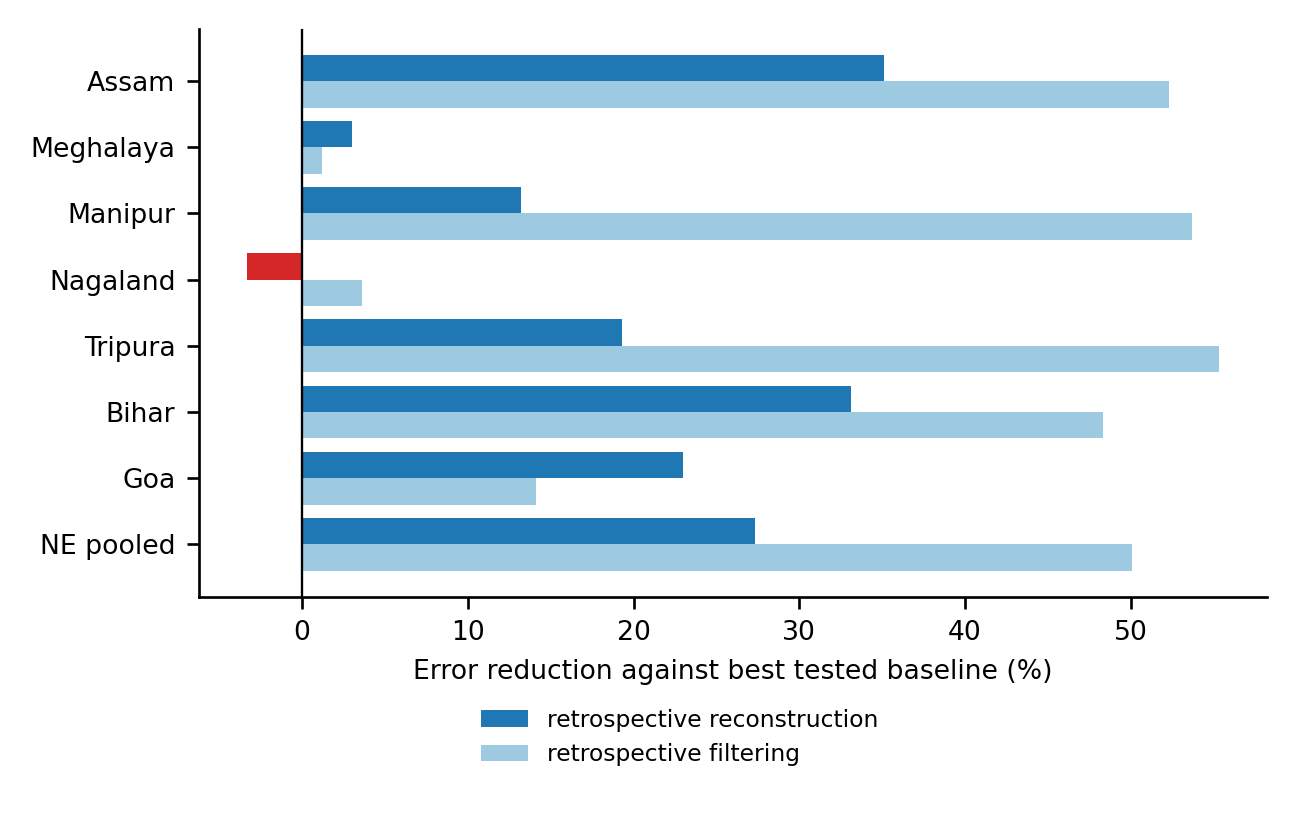
\includegraphics[width=\linewidth]{fig_gain_audited.png}
\caption{Relative error reduction over the best tested baseline in each state. The filtered-state series uses retrospective full-panel fits; it is not a nowcasting result. Negative values indicate higher error.}
\Description{Paired horizontal bars show retrospective reconstruction and filtered-state relative error reductions across states and the North-East pool.}
\label{fig:gain}
\end{figure}
\end{minipage}\hfill
\begin{minipage}[t]{0.49\linewidth}\vskip0pt\relax
\begin{figure}
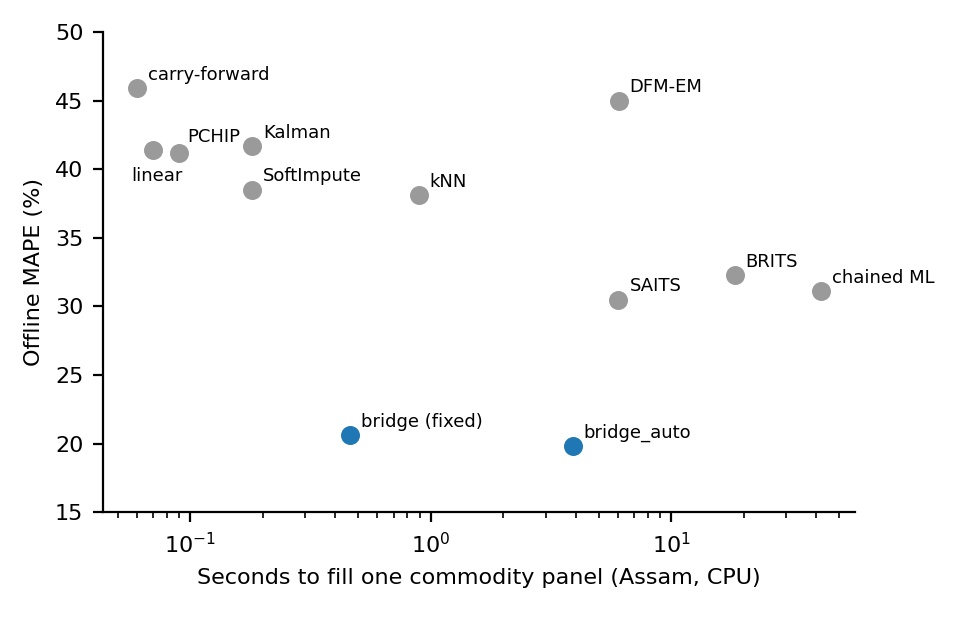
\includegraphics[width=\linewidth]{fig_cost.png}
\caption{Assam retrospective MAPE against measured fill time per commodity panel (one CPU core; logarithmic time axis). These are configuration-specific measurements, not model-family complexity bounds.}
\Description{Scatter plot of error against runtime for the twelve tested implementations, with fixed and adaptive bridges highlighted.}
\label{fig:cost}
\end{figure}
\end{minipage}

\noindent\begin{minipage}[t]{0.49\linewidth}\vskip0pt\relax
\begin{figure}
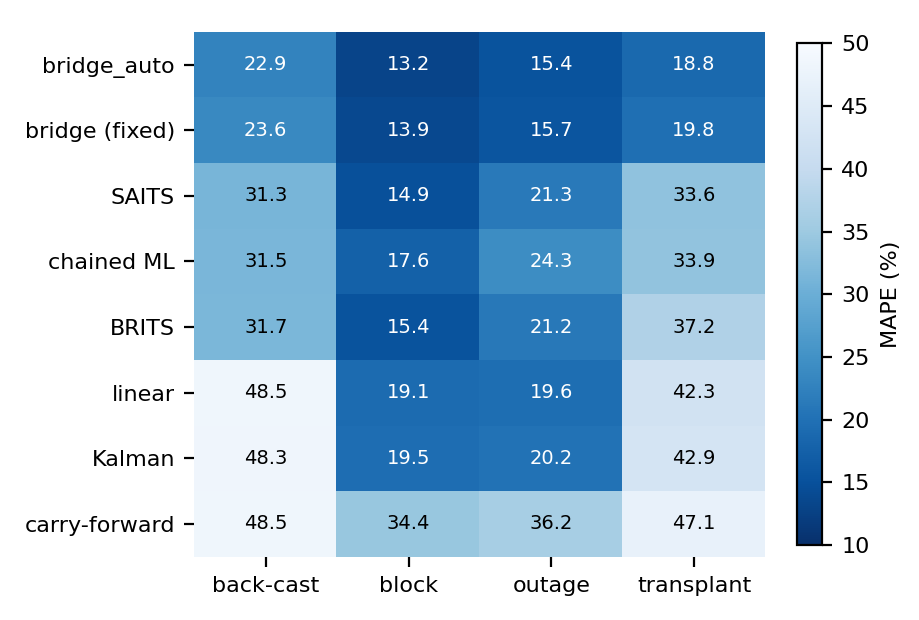
\includegraphics[width=0.94\linewidth]{fig_scenarios.png}
\caption{Assam retrospective MAPE by saved scenario. Block and outage entries correspond to the displayed heavy-method comparison runs, not accuracy in genuinely unreported weeks.}
\Description{Heat map of errors for eight implementations across back-cast, block, outage and transplant scenarios.}
\label{fig:scenarios}
\end{figure}
\end{minipage}\hfill
\begin{minipage}[t]{0.49\linewidth}\vskip0pt\relax
\begin{figure}
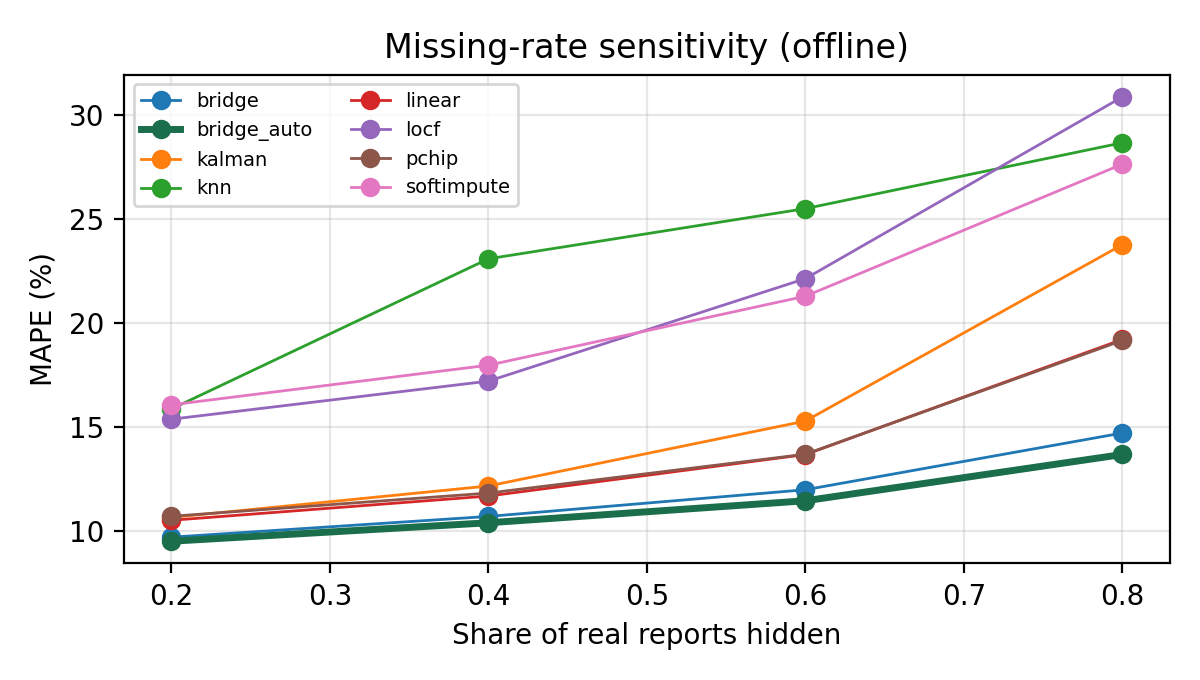
\includegraphics[width=\linewidth]{missing_rate.png}
\caption{Assam error under additional random deletion of reported values. The 20--80\% masking sweep is distinct from the naturally occurring missingness mechanism.}
\Description{Error curves for selected methods as the proportion of deliberately hidden observed reports increases.}
\label{fig:missing}
\end{figure}
\end{minipage}

